\documentclass[12pt]{article}
% \usepackage{arxiv}


\usepackage[colorlinks=true,linkcolor=blue]{hyperref}

\textheight=24cm
\textwidth=16cm
\oddsidemargin=5mm
\evensidemargin=-5mm
\marginparwidth=36pt
\topmargin=-2cm
\footskip=2.5em
\footnotesep=2ex




\usepackage[utf8]{inputenc}
\usepackage[english, russian]{babel}
\usepackage[T1]{fontenc}
\usepackage{url}
\usepackage{booktabs}
\usepackage{tabularx}
\usepackage{amsfonts}
\usepackage{nicefrac}
\usepackage{microtype}
\usepackage{lipsum}
\usepackage{graphicx}
\usepackage{natbib}
\usepackage{doi}

\usepackage{svg}

\usepackage{multirow}
\usepackage{ragged2e}
\usepackage{indentfirst}
\usepackage{multicol}
\usepackage{subfig}
\usepackage{amsmath,amssymb}
\usepackage{enumerate}
\usepackage{mathtools}
\usepackage{comment}
\usepackage{multicol}

\graphicspath{ {./images/} }

\title{Выделение графовых структур в тексте с помощью больших языковых моделей}

\author{ Левыкин Александр Михайлович \\
        Факультет вычислительной математики и кибернетики \\
        МГУ им. Ломоносова \\
        \texttt{melikhov.dmitry.a@gmail.com} \\
	%% examples of more authors
	\And
	Воронцов Константин Вячеславович \\
        Факультет вычислительной математики и кибернетики \\
        МГУ им. Ломоносова \\
        \texttt{vokov@forecsys.ru} \\
}
\date{}

% \renewcommand{\shorttitle}{\textit{arXiv} Template}

%%% Add PDF metadata to help others organize their library
%%% Once the PDF is generated, you can check the metadata with
%%% $ pdfinfo template.pdf
\hypersetup{
pdftitle={A template for the arxiv style},
pdfsubject={q-bio.NC, q-bio.QM},
pdfauthor={David S.~Hippocampus, Elias D.~Striatum},
pdfkeywords={First keyword, Second keyword, More},
}

\begin{document}

\begin{titlepage}
\begin{center}
    

    \bigskip
    
\includegraphics[width=50mm]{msu.eps}

    \bigskip
    Московский государственный университет имени М.В. Ломоносова
    Факультет Вычислительной Математики и Кибернетики \\
    Кафедра Математических Методов Прогнозирования \\
    \bigskip
    \bigskip
    \bigskip
    \bigskip
    \bigskip
    {\large Левыкин Александр Михайлович} \\
    \bigskip
    \bigskip
    \textsf{\Large\bfseries
        Детекция галлюцинаций больших языковых моделей \\[10mm]
    }\\[10mm]
    ВЫПУСКНАЯ КВАЛИФИКАЦИОННАЯ РАБОТА \\[50mm]
    \begin{flushright}
        \parbox{0.3\textwidth}{
            % Выполнил:\\
            % студент 4 курса 417 группы\\
            % \emph{Мелихов Дмитрий Александрович}\\[5mm]
            Научный руководитель:\\
            д.ф.-м.н., профессор\\
            \emph{Воронцов К.В.}
        }
    \end{flushright}

    % \begin{tabular}{p{0.45\textwidth}p{0.45\textwidth}}
    %     Заведующий кафедрой\newline
    %     Математических Методов\newline
    %     Прогнозирования, профессор РАН
    %     &
    %     ~\newline~\newline
    %     \hfill\hbox to 0.45\textwidth{\hrulefill \hspace{1em} К.В. Воронцов}
    % \\[20mm]
    %     К защите допускаю\newline
    %     \hbox to 0.4\textwidth{<<\hbox to 12mm{\hrulefill}>> \hrulefill \hspace{1em} 2024.}
    %     &
    %     К защите рекомендую \newline
    %     \hbox to 0.45\textwidth{<<\hbox to 12mm{\hrulefill}>> \hrulefill \hspace{1em} 2024.}
    % \end{tabular}

    \vspace{\fill}
    Москва, 2025
\end{center}
\end{titlepage}

\clearpage
\tableofcontents
\clearpage

\begin{abstract}
В данной работе рассматривается задача детекции галлюцинаций больших языковых моделей. Основное внимание уделяется решению задачи в token classification постановке, в которой требуется классифицировать на наличие галлюцинаций каждый токен ответа модели. Анализируются подходы instruction-based, дообучение NER моделей, RAG подход, а также анализ временных рядов. Рассматривается новая постановка задачи с добавлением в целевые фрагменты вероятностей, с которыми они являются галлюцинациями, и соответствующие новые критерии оценки качества моделей детекции.

%В данной работе рассматривается задача выделения связей в тексте на примере данных scierc. Сравниваются различные векторные представления фрагментов текста для классификации связей. Представляется модход MRC для классификации связей между фрагментами. Для задачи совместного выделения фрагментов и связей представляется новый критерий оценивания, который учитывает неточности выделения фрагментов и неточности классификации связей. Данный критерий сглаживает F-меру и ослабляет требования.
%
\end{abstract}


\section{Введение}
\subsection{Цель исследования и его мотивация}
Современные большие языковые модели (БЯМ) демонстрируют значительные успехи в различных задачах обработки естественного языка, включая генерацию текстов, машинный перевод и понимание контекста. Однако, несмотря на впечатляющие достижения, одним из основных недостатков таких моделей является склонность к генерации недостоверной информации, известной как «галлюцинации». Галлюцинации БЯМ представляют собой фрагменты текста, которые модель создает, основываясь не на фактических данных или правдоподобной логике, а на случайных ассоциациях, что может привести к искажению смысла или созданию ложной информации. Это представляет серьёзную проблему при использовании БЯМ в критически важных областях, таких как медицина, право и научные исследования, где достоверность информации является ключевой.

Цель данного исследования заключается в разработке и оценке методов, направленных на детекцию галлюцинаций на уровне отдельных токенов в сгенерированных БЯМ текстах. Это позволит значительно улучшить качество генерации текста, повысить уровень доверия к результатам работы моделей и обеспечить более надёжное их применение в практических задачах. Мотивация данного исследования обусловлена необходимостью минимизировать негативные последствия ошибок БЯМ и сделать их более прозрачными и безопасными для использования.
\subsection{Объект исследования}
Объектом исследования в данной работе являются галлюцинации больших языковых моделей. Термин «галлюцинация» в данном контексте обозначает неточности или ложные утверждения, которые возникают в сгенерированном модели тексте, не имеющие опоры на фактическую информацию или логическое обоснование. Под «детекцией галлюцинаций» понимается процесс идентификации этих ошибок в тексте, с классификацией каждого токена по вероятности того, что он является галлюцинацией.

Кроме того, в работе используются следующие термины:

Token Classification — задача классификации, в которой каждый токен (элемент текста, обычно слово или символ) оценивается по наличию или отсутствию определённого признака, в данном случае — галлюцинации.
Instruction-based подходы — подходы, основанные на задавании модели конкретных инструкций для выполнения задач, что может включать и детекцию ошибок.
NER модели (Named Entity Recognition) — модели, предназначенные для распознавания именованных сущностей, которые можно адаптировать для выявления галлюцинаций.
RAG подход (Retrieval-Augmented Generation) — гибридный метод, сочетающий генерацию текста с извлечением информации из внешних источников для повышения точности ответа.

\subsection{Актуальные проблемы}
Одной из ключевых проблем, связанных с большими языковыми моделями, является их склонность к генерации галлюцинаций — фрагментов текста, которые не соответствуют фактическим данным или контексту задачи. Галлюцинации могут проявляться в разных формах, включая ложные утверждения, вымышленные факты и искажение исходной информации. Это явление особенно опасно в ситуациях, где требуется высокая степень точности и достоверности, таких как медицинские заключения, юридические документы или научные исследования.

Основная сложность заключается в том, что галлюцинации не всегда очевидны для конечного пользователя и могут возникать даже при кажущейся логичности и правдоподобности ответа модели. Большие языковые модели, такие как GPT или BERT, обучены на огромных наборах данных и часто полагаются на вероятностные подходы для генерации текста, что делает их поведение труднопредсказуемым. В результате, галлюцинации могут возникать даже при корректном вводе данных, и выявление таких ошибок требует разработки специализированных методов и подходов.

Кроме того, существующие методы детекции галлюцинаций сталкиваются с рядом вызовов. Во-первых, галлюцинации могут быть контекстно зависимыми, и выявить их на уровне отдельных токенов (слов или символов) представляет сложную задачу. Во-вторых, не существует единой чёткой методики для оценки качества детекции галлюцинаций, так как в различных ситуациях модели могут демонстрировать различные типы ошибок. Это усложняет разработку и тестирование моделей, способных эффективно выявлять галлюцинации с высокой точностью и надёжностью.

Таким образом, основная проблема заключается в разработке метода, который сможет точно и эффективно классифицировать каждый токен текста на предмет наличия галлюцинаций.

\subsection{Обзор литературы}
1. Combinatorial Testing для детекции галлюцинаций в медицине
Исследование Perko, Wotawa и Nica (2024) посвящено применению **комбинаторного тестирования** для детекции галлюцинаций, сгенерированных большими языковыми моделями (БЯМ) в медицинских контекстах. Авторы демонстрируют, как такие методы могут эффективно выявлять галлюцинации в медицинских ответах, которые имеют критически важное значение. Этот подход отличается тем, что использует комбинации возможных параметров и тестов для генерации ответов модели и последующей проверки их на соответствие реальной информации. [Источник]\url{https://is.ijs.si/wp-content/uploads/2024/09/IS2024_-_CHATGPT_in_MEDICINE_paper_10.pdf}

2. **Sanitizing LLMs для обнаружения багов**  
Wang et al. (2024) исследовали новую технику санитизации (очистки) для предотвращения галлюцинаций при обнаружении багов в программировании. Их метод основан на проверке путей передачи данных (data-flow) и позволяет улучшить детекцию ошибок в коде. Это подчеркивает универсальность подходов детекции галлюцинаций, поскольку они могут быть применимы не только в языковых задачах, но и в технических контекстах, таких как обнаружение уязвимостей. [Источник](https://chengpeng-wang.github.io/publications/LLMSAN_EMNLP2024.pdf)

3. **Auto-GDA: Адаптация моделей для верификации фактов**  
Leemann et al. (2024) предложили **автоматическую доменную адаптацию** для улучшения верификации фактов в Retrieval-Augmented Generation (RAG) подходах. Этот метод призван уменьшить количество галлюцинаций в текстах, сгенерированных БЯМ, путем автоматической адаптации к конкретным доменам и верификации через внешние источники данных. Это направление исследований показывает эффективность гибридных моделей, которые сочетают генерацию текста с проверкой фактов. [Источник](https://arxiv.org/pdf/2410.03461)

4. **HaloScope: Использование несупервизированных генераций для детекции галлюцинаций**  
В работе Du, Xiao и Li (2024) представлено решение **HaloScope**, которое использует несупервизированные генерации больших языковых моделей для выявления галлюцинаций. Метод использует динамическое обучение на большом объеме данных, чтобы оценивать вероятность того, что сгенерированный текст содержит галлюцинации, без необходимости использования маркированных данных. Этот подход позволяет автоматизировать детекцию галлюцинаций в неструктурированных данных. [Источник](https://arxiv.org/pdf/2409.17504)

5. **MedHalu: Детекция галлюцинаций в медицинских запросах**  
Agarwal et al. (2024) в своем исследовании фокусируются на медицинских галлюцинациях, возникающих в ответах на запросы к БЯМ в медицинских контекстах. Авторы предложили экспертно ориентированный подход, при котором модель обучается на основе обратной связи от экспертов для улучшения качества детекции галлюцинаций. Это особенно важно в медицинских задачах, где неточные ответы могут иметь серьезные последствия. [Источник](https://arxiv.org/pdf/2409.19492)

Таким образом, обзор литературы показывает, что подходы к детекции галлюцинаций в БЯМ активно развиваются и охватывают различные области, начиная от медицины и заканчивая программированием. Среди наиболее перспективных методов выделяются гибридные подходы (RAG), использующие внешние данные для проверки фактов, а также техники безразметочного обучения, которые позволяют адаптироваться к большим объемам данных без ручной разметки.

\subsection{Предлагаемое решение}
В данной работе проводятся эксперименты с instruction-based методами использования заранее обученных моделей. Кроме того, рассматривается подход анализа логитов сгенерированного текста, что позволяет полностью отказаться от информации о словах и языке. Такой подход не рассматривался в обозреваемых работах.

\subsection{Инструменты и процесс работы}
Для проведения экспериментов использовалась платформа Kaggle, которая предоставила вычислительные мощности, включая графический процессор (GPU) NVIDIA P100 с 16 Gb видеопамяти. Выбор Kaggle для реализации экспериментов был обусловлен возможностью быстрой настройки среды, доступа к широкому набору библиотек для машинного обучения и удобства совместного использования кода и результатов.

\clearpage
\section{Постановка задачи}

Задача выделения фрагментов галлюцинаций в тексте представляет собой задачу классификации токенов, в которой каждому токену присваивается метка, указывающая, является ли он частью галлюцинации или нет. Для решения этой задачи используется формат BIO-разметки (отмечающий начало, середину и конец фрагментов, содержащих галлюцинации). Формат BIO позволяет более точно определять начало и границы фрагментов и показывает лучшие результаты в сравнении с форматом бинарной классификации каждого токена. В данном разделе мы подробно опишем задачу обучения модели и введем основные обозначения.

\subsection*{Формализация задачи}

Рассмотрим текст, состоящий из \( N \) токенов, представленных последовательностью \( X = (x_1, x_2, \ldots, x_N) \). Модель должна классифицировать каждый токен \( x_i \) как принадлежащий галлюцинации или нет, используя BIO-формат, где:
\begin{itemize}
\item \textbf{B} обозначает начало фрагмента галлюцинации,
\item \textbf{I} обозначает токен, продолжающий галлюцинацию,
\item \textbf{O} обозначает токен, не связанный с галлюцинацией.
\end{itemize}
Для этого модель обучается предсказывать вероятности \( \hat{S} \) для каждого токена текста.

\textbf{Обозначения матриц меток и предсказаний:}

\( S \in \{0, 1\}^{N \times 3} \): бинарная матрица, содержащая истинные метки для каждого токена, где:
   \begin{itemize}
     \item \( S_{i,0} = 1 \), если токен \( x_i \) отмечен как \textbf{B},
     \item \( S_{i,1} = 1 \), если токен \( x_i \) отмечен как \textbf{I},
     \item \( S_{i,2} = 1 \), если токен \( x_i \) отмечен как \textbf{O}.
   \end{itemize}
\( \hat{S} \in [0, 1]^{N \times 3} \): матрица предсказаний модели, где \( \hat{S}_{i,t} \) обозначает вероятность того, что токен \( x_i \) относится к классу \( t \in \{ B, I, O \} \).

\textbf{Ограничения нормировки:}

   Для каждого токена модель должна предсказывать распределение вероятностей по трем меткам, что выражается следующим условием:
   $$
   \sum_t \hat{S}_{i, t} = 1, \quad \forall i \in \{1, \dots, N\}
   $$

\textbf{Функция потерь — кросс-энтропия:}

   Для оптимизации параметров span-detection моделей используется функция потерь на основе кросс-энтропии, которая минимизируется по параметрам модели \( \theta' \):
   $$
   CE(S, \hat{S}) = -\frac{1}{N} \sum_{i=1}^{N} \sum_{t \in \{B, I, O\}} S_{i, t} \log(\hat{S}_{i, t})
   $$
   Здесь:
   - \( S_{i, t} \) — бинарный индикатор для истинной метки токена \( x_i \) по классу \( t \),
   - \( \hat{S}_{i, t} \) — вероятность, предсказанная моделью для метки \( t \) токена \( x_i \).

И задача обучения модели заключается в поиске параметров, доставляющих минимум функции потерь:
$$
CE(S, p(S \mid \theta)) = CE(S, \hat{S}) = -\frac{1}{N} \sum_{i=1}^{N} \sum_{t \in \{B, I, O\}} S_{i, t} \log(\hat{S}_{i, t}) \longrightarrow \min_{\theta}
$$

\clearpage
\section{Метод решения}
\subsection{Instruction-based подход}
\subsection{Обучение рекуррентной нейросети LSTM}

\clearpage
\section{Данные}


\clearpage
\section{Критерии качества модели}

Для оценки качества модели для выделения тегированных фрагментов во многих работах используется $F_1 score$ с микро усреднением (NER micro $F_1$). По всей выборке для каждого тега считается матрица ошибок, усредняются по тегам и считается среднее гармоническое полученных точности и полноты.

Для оценки качества классификации связей используется $F_1 score$ с макро усреденением (Rel macro $F_1$): усредняются точность и полнота для каждого класса. Для оценки качества выделения связей используется $F_1 score$ с микро усреденением (Rel micro $F_1$): объект считается правильно выделенным, если правильно выделены и оба фрагмента и отношение.

Для оценки совместной классификации используется ослабленный $F_1 score$ с микро усреднением (Rel Soft micro $F_1$): считается как Rel micro $F_1$ c поправкой на неточность выделения фрагментов и неточность классификации связей. Подробный алгоритм вычисления можно найти в приложении. Данная величина позволяет рассмотреть только качество выделение пар фрагментов, между которыми есть связь.
\clearpage
\section{Эксперименты}
Эксперименты проводятся на видеокарте NVIDIA GeForce RTX 3090, фиксируется random seed = 42, batch\_size = 4, learning\_rate = $2e^{-5}$, для получения векторного представления используется предобученная модель allenai/scibert\_scivocab\_uncased.

Во время обучения каждые 25 итераций из 87 в эпохе замеряется качество на валидационной выборке. Для тестовой выборки выбирается итерация, которая показала максимальное значение на критерии Rel micro $F_1$ на валидационной выборке.

\subsection{Выделение связей с известными связями}
Графики обучения представлены на рисунках \ref{fig:loss_clf}, \ref{fig:grad_clf}, \ref{fig:f_clf_rel_clf}, \ref{fig:f_rel_rel_clf}. Результат обучения нахождения связей с известными фрагментами представлен в таблице \ref{table:res_clf}. Лучший результат по micro $F_1$ получился для MRC и усреднения с помощью механизма внимания. Сильное различие между микро и макро усреднением (с учётом того, как они считались) объясняется низким качеством поиска релевантных пар среди известных.

\begin{table}[h!]
\centering
\begin{tabular}{| c || p{2cm} | p{2cm} || p{2cm} | p{2cm} |} 
 \hline
 Модель & Valid Rel micro $F_1$ & Valid Rel macro $F_1$ & Test Rel micro $F_1$ & Test Rel macro $F_1$  \\ [0.5ex] 
 \hline\hline
 Base + EndsPool & 0.39 & \textbf{0.78} & 0.43 & \textbf{0.72} \\ 
 \hline
 Base + MeanPool & 0.38 & 0.73 & 0.37 & 0.70 \\ 
 \hline
 Base + AttentionPool & 0.39 & 0.76 & 0.43 & 0.72 \\ 
 \hline
 MRC + EndsPool & 0.41 & 0.72 & 0.40 & 0.70 \\ 
 \hline
 MRC + MeanPool & 0.42 & 0.74 & 0.43 & 0.68  \\ 
 \hline
 MRC + AttentionPool & \textbf{0.46} & 0.71 & \textbf{0.48} & 0.71
 \\[1ex] 
 \hline
\end{tabular}
\vspace{1ex}
\caption{Результат обучения нахождения связей с известными фрагментами.}
\label{table:res_clf}
\end{table}

\subsection{Совместное выделение фрагментов и связей}

Результаты совместного выделения фрагментов и связей представлена в таблице \ref{table:res_joint}. Модель для выделения именованных сущностей показывает качество 0.93 для микро усреденения и 0.89 для макро усредения $F_1$. Лучший результат получился для MRC: по $F_1$ с микро усредением лучший для векторного представления фрагмента как среднего векторных представлений слов, по ослабленному критерию для усредения через механизм внимания.

\begin{table}[h!]
\centering
\begin{tabular}{| c || p{2cm} | p{2cm} |} 
 \hline
 Модель & Test Rel micro $F_1$ & Test Rel Soft macro $F_1$  \\ [0.5ex] 
 \hline\hline
 Base + EndsPool & 0.0006 & 0.022 \\ 
 \hline
 Base + MeanPool & 0.0008 & 0.022 \\
  \hline
 Base + AttentionPool &  0.0005 & 0.026\\ 
 \hline
 MRC + EndsPool & 0.0 & 0.028\\ 
 \hline
 MRC + MeanPool & \textbf{0.0012} & 0.028\\ 
 \hline
 MRC + AttentionPool & 0.0 & \textbf{0.039}\\[1ex] 
 \hline
\end{tabular}
\vspace{1ex}
\caption{Результат обучения совместного выделения фрагментов и связей.}
\label{table:res_joint}
\end{table}
% \begin{table}[h!]
% \centering
% \begin{tabular}{| c || p{2cm} | p{2cm} |} 
%  \hline
%  Модель & Test NER micro $F_1$ & Test NER macro $F_1$ & Test Rel micro $F_1$ & Test Rel Soft macro $F_1$  \\ [0.5ex] 
%  \hline\hline
%  Base + EndsPool & 0.92 & 0.88 & 0.0006 & 0.022 \\ 
%  \hline
%  Base + MeanPool & \textbf{0.93} & \textbf{0.89} & 0.0008 & 0.022 \\
%   \hline
%  Base + AttentionPool & \textbf{0.93} & \textbf{0.89} &  0.0005 & 0.026\\ 
%  \hline
%  MRC + EndsPool & 0.84 & 0.71 & 0.0 & 0.028\\ 
%  \hline
%  MRC + MeanPool & 0.82 & 0.67 & \textbf{0.0012} & 0.028\\ 
%  \hline
%  MRC + AttentionPool & 0.86 & 0.75 & 0.0 & \textbf{0.039}\\[1ex] 
%  \hline
% \end{tabular}
% \vspace{1ex}
% \caption{Результат обучения совместного выделения фрагментов и связей.}
% \label{table:res_joint}
% \end{table}

\clearpage
\section{Вывод}

В данной работе были рассмотрены разные векторные представления фрагментов для задачи классификации связей, а также рассмотрен подход MRC. В результате экспериментов самым лучшим по $F_1$ с микро усреднением оказался метод MRC с векторным представлением фрагментов, которое строится усреднением через механизм внимания.

Был предложен критерий оценки качества моделей для совместного выделения сущностей и фрагментов, который сглаживает F-меру и позволяет лучше оценить качество разметки. Лучший результат показал подход MRC.
Основная проблемма методов - низкое качество поиска релевантных пар фрагментов.

Дальнейшая работа связана с улучшением качества совместного выделения фрагментов и связей между ними.
\clearpage
\bibliographystyle{splncs04}
\bibliography{references}

\clearpage
\section{Приложение}

\subsection{Вычисление критериев качества моделей}

NER metrics:
$$
SpanTP = \sum_i^N [arg\max_j(\hat{S}_{i, j}) = S_i]
$$
$$
SpanTP_k = \sum_i^N [arg\max_j(\hat{S}_{i, j}) = S_i = k]
$$
$$
SpanF_k = \sum_i^N [arg\max_j(\hat{S}_{i, j}) \neq S_i]
$$
$$
SpanFP_k = \sum_i^N [k = arg\max_j(\hat{S}_{i, j}) \neq S_i]
$$
$$
SpanFN_k = \sum_i^N [arg\max_j(\hat{S}_{i, j}) \neq S_i = k]
$$
\begin{center}
\boxed{$$
NER~micro~F_1 = \frac{2 \cdot SpanTP}{2 \cdot SpanTP + SpanF}
$$}
\end{center}
$$
SpanRecall = mean_k\{ \frac{SpanTP_k}{ SpanTP_k + SpanFN_k} \}
$$
$$
SpanPrecision = mean_k\{ \frac{SpanTP_k}{ SpanTP_k + SpanFP_k} \}
$$
\begin{center}
\boxed{$$
NER~macro~F_1 = \frac{2 \cdot SpanRecall * SpanPrecision}{SpanRecall + SpanPrecision}
$$}
\end{center}

Relation metrics:

$Rel~macro~F_1$ вычисляется аналогично $NER~macro~F_1$.

Пусть $Rel$ - четвёрки из выборки $(s1, e1, s2, e2, r)$ - начала и концы фрагментов и отношение между ними. $\hat{Rel}$ - предсказанные четвёрки.

\begin{center}
\boxed{$$Rel~micro~F_1 = \frac{2 \cdot |Rel \cap \hat{Rel}|}{|Rel| + |\hat{Rel}|}$$}
\end{center}

$IoU(a_1, a_2, b_1, b_2)$ - отношение мощности пересечения к мощности объединения для 2 отрезков: $(a_1, a_2),~(b_1, b_2)$

$$
SoftIntersection(a, b) = 
% \begin{cases}
\frac{1}{2} (IoU(a_1, a_2, b_1, b_2) + IoU(a_3, a_4, b_3, b_4))
% \text{ if } a_5 \neq 0, b_5 \neq 0\\
% IoU(a_1, a_2, b_1, b_2) * IoU(a_3, a_4, b_3, b_4) \text{ if } a_5 = b_5 \\
% 0 \text{ o.w.}
% \end{cases}
$$

$$
SoftIntersection(Rel, \hat{Rel}) = \max_{I} \sum_{(i, j) \in I} SoftIntersection(Rel_i, \hat{Rel}_j).
$$
Где I - множества пар, такие что $\forall i \neq j$, $i, j \leq |I|$: $I_{i, 0} \neq I_{j, 0}$ и $I_{i, 1} \neq I_{j, 1}$.


\begin{center}
\boxed{$$Rel~Soft~micro~F_1 = \frac{2 \cdot SoftIntersection(Rel, \hat{Rel})}{|Rel| + |\hat{Rel}|}$$}
\end{center}


\subsection{Графики обучения}

\begin{figure}[h]
    \centering
    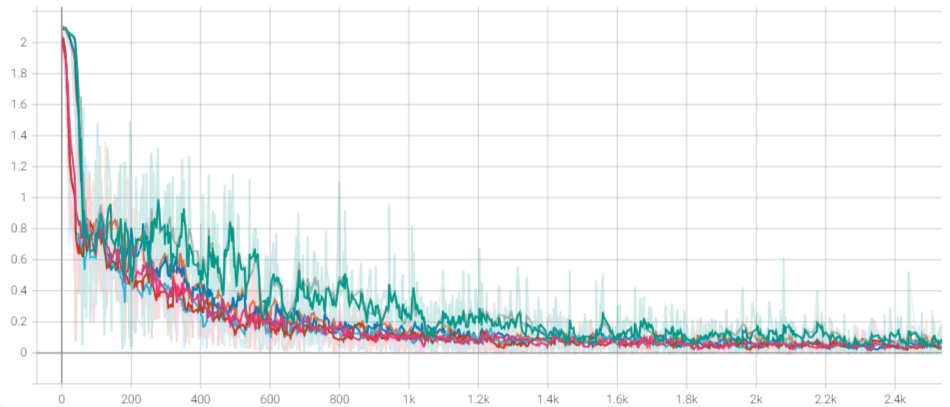
\includegraphics[width=\textwidth]{loss.png}
    \caption{Функция потерь в зависимости от итерации. Обучение нахождения связей с известными фрагментами.}
    \label{fig:loss_clf}
\end{figure}

\begin{figure}[h]
    \centering
    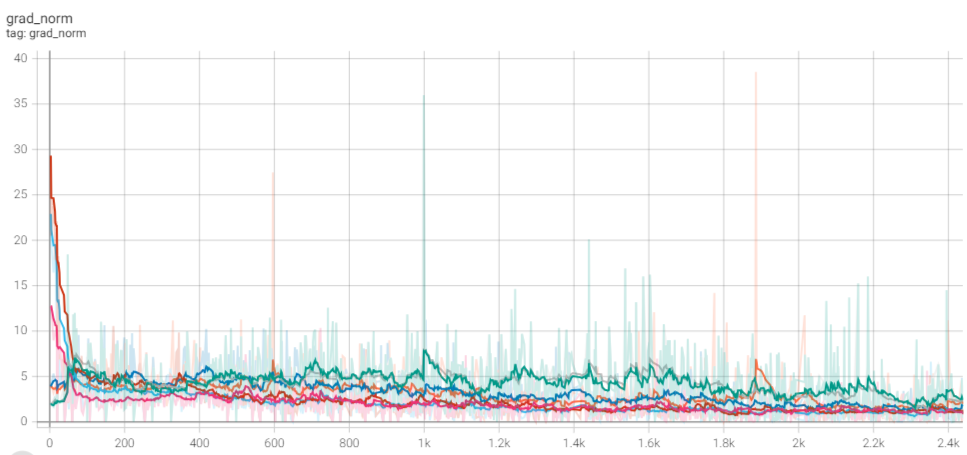
\includegraphics[width=\textwidth]{images/grad_norm.png}
    \caption{Норма градиента в зависимости от итерации. Обучение нахождения связей с известными фрагментами.}
    \label{fig:grad_clf}
\end{figure}

\begin{figure}[h]
    \centering
    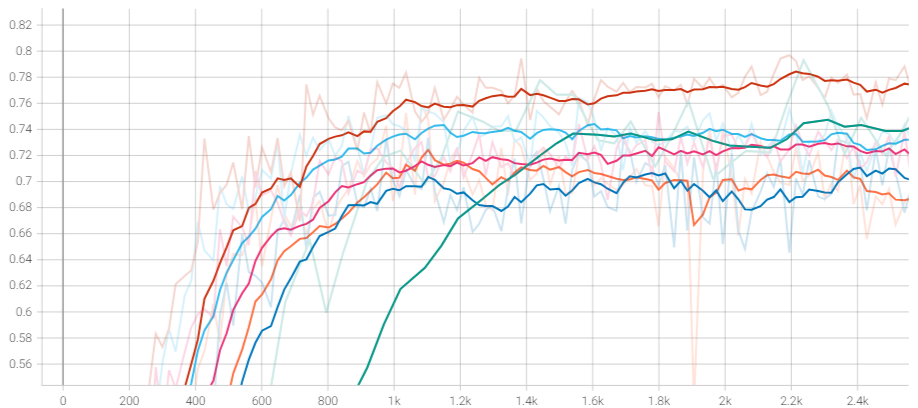
\includegraphics[width=\textwidth]{images/f_clf.png}
    \caption{$macro F_1$ на валидационной выборке для задачи классификации связей в зависимости от итерации. Обучение нахождения связей с известными фрагментами.}
    \label{fig:f_clf_rel_clf}
\end{figure}

\begin{figure}[h]
    \centering
    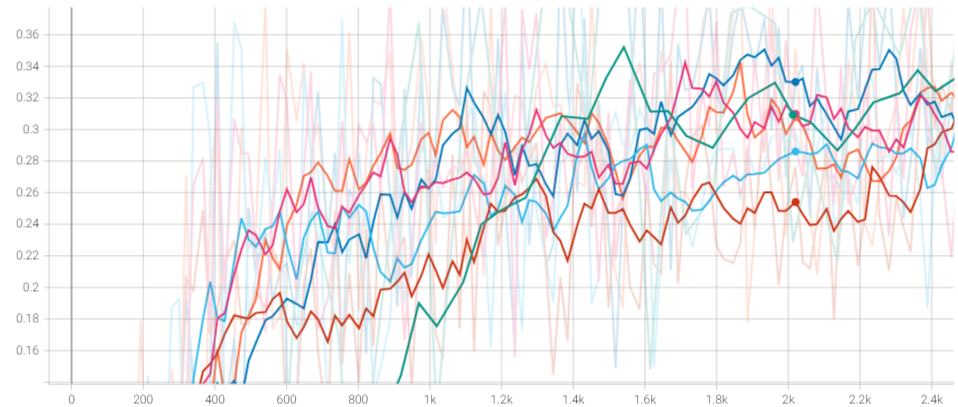
\includegraphics[width=\textwidth]{images/f_rel.png}
    \caption{$micro F_1$ на валидационной выборке для задачи нахождения связей в зависимости от итерации. Обучение нахождения связей с известными фрагментами.}
    \label{fig:f_rel_rel_clf}
\end{figure}

\begin{figure}[h]
    \centering
    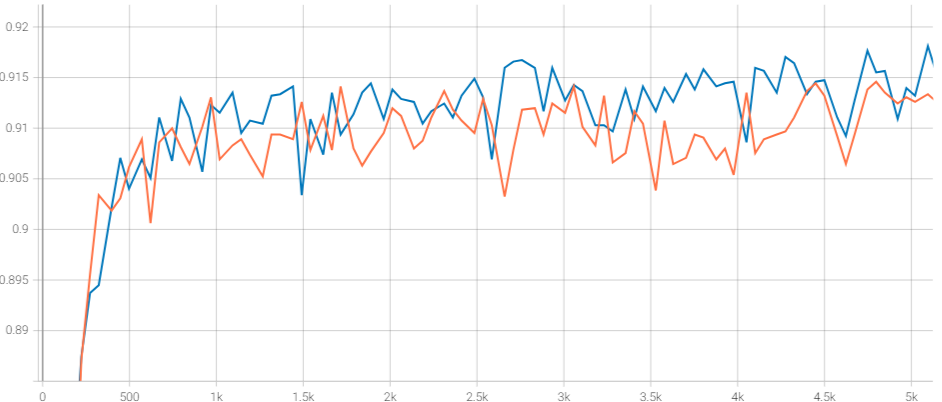
\includegraphics[width=\textwidth]{images/ner_micro_f1.png}
    \caption{NER $micro F_1$ на валидационной выборке в зависимости от итерации для задачи нахождения связей. Обучение совместного нахождения фрагментов и связей между ними.}
    \label{fig:ner_micro_f}
\end{figure}

\begin{figure}[h]
    \centering
    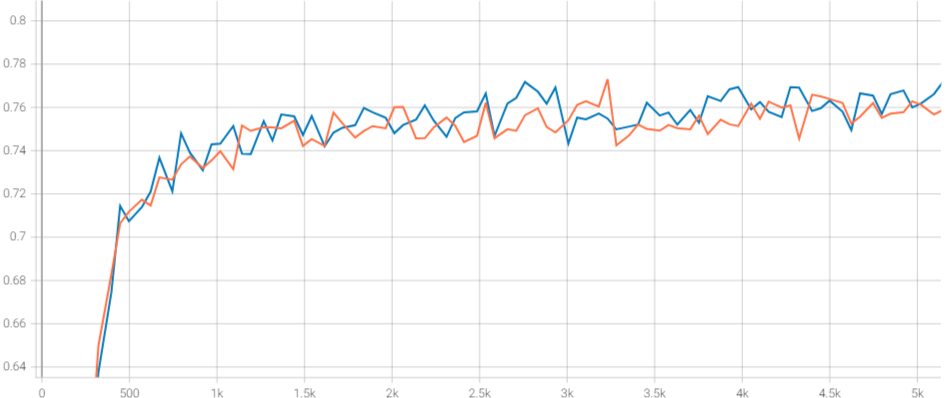
\includegraphics[width=\textwidth]{images/ner_macro_f1.png}
    \caption{NER $macro F_1$ на валидационной выборке в зависимости от итерации для задачи нахождения связей. Обучение совместного нахождения фрагментов и связей между ними.}
    \label{fig:ner_macro_f}
\end{figure}

\begin{figure}[h]
    \centering
    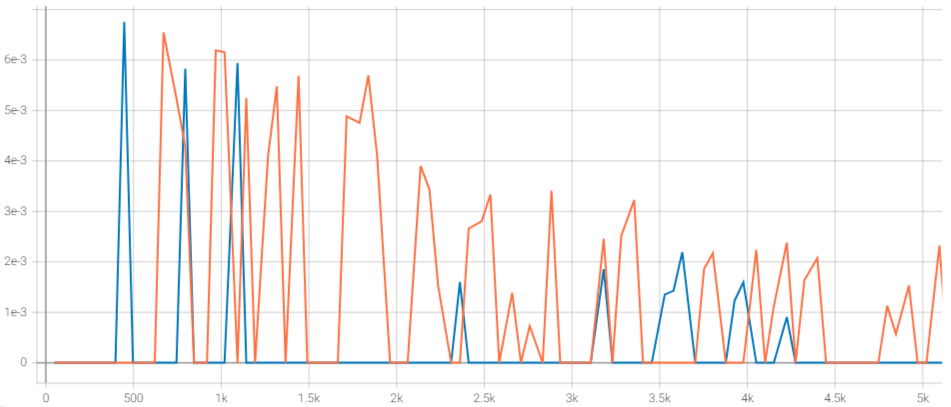
\includegraphics[width=\textwidth]{images/hard_rel_f1.png}
    \caption{Rel $micro F_1$ на валидационной выборке в зависимости от итерации для задачи нахождения связей. Обучение совместного нахождения фрагментов и связей между ними.}
    \label{fig:ner_micro_f}
\end{figure}

\begin{figure}[h]
    \centering
    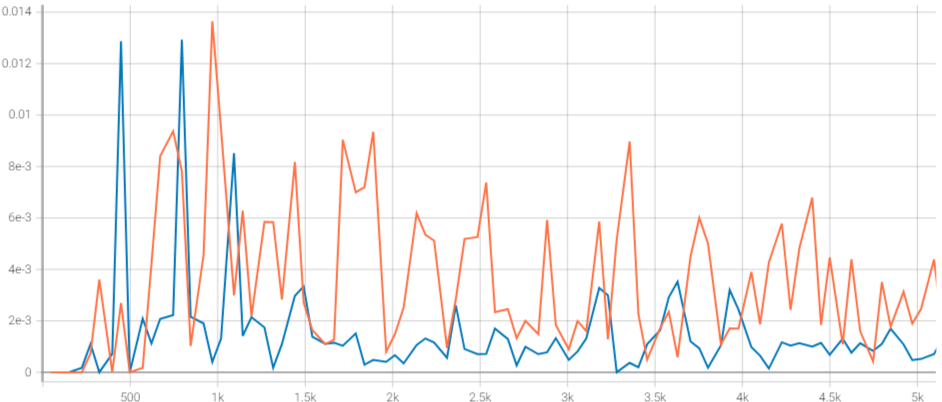
\includegraphics[width=\textwidth]{images/smooth_rel_f1.png}
    \caption{Soft $micro F_1$ на валидационной выборке в зависимости от итерации для задачи нахождения связей. Обучение совместного нахождения фрагментов и связей между ними.}
    \label{fig:ner_micro_f}
\end{figure}

\end{document}